\documentclass[10pt,a4paper]{scrartcl}
\PassOptionsToPackage{table}{xcolor}
\usepackage[utf8]{inputenc}
\usepackage[T1]{fontenc}
\usepackage[ngerman]{babel}
\usepackage{microtype, multicol, marginnote, bera, parskip}
\usepackage{listings, amsmath, amssymb, graphicx, tikz, epic}
\usepackage{stmaryrd} %for lightning arrow
\usepackage{pstricks, pst-node, pst-tree, pdflscape}
\usepackage[babel=true]{csquotes}
\usepackage{placeins}
\usepackage[labelformat=empty]{caption}
\tolerance=2000
\setcounter{secnumdepth}{0}
\usepackage[inner=2cm,outer=2cm,top=1.5cm,bottom=1.5cm,includeheadfoot]{geometry}
\usepackage{multirow}
\newcommand{\subExercise}[1]{\vspace{0.5em} \noindent{\bf #1)}}
\newcommand{\B}{\mathbb{B}}
\DeclareMathOperator{\op}{op}

\author{Michael Mardaus \and Andrey Tyukin}
\title{
\includegraphics[scale=0.2]{../logo_schriftzug}\\
Technische Informatik: Abgabe 8}

\begin{document}

\maketitle

\section*{Exercise 8.1 (JK Flipflop ringcounter)}
Let FF1 be a $0\rightarrow 1$ flank controlled D-flipflop and FF2 a $1\rightarrow0$ flank controlled one.\\
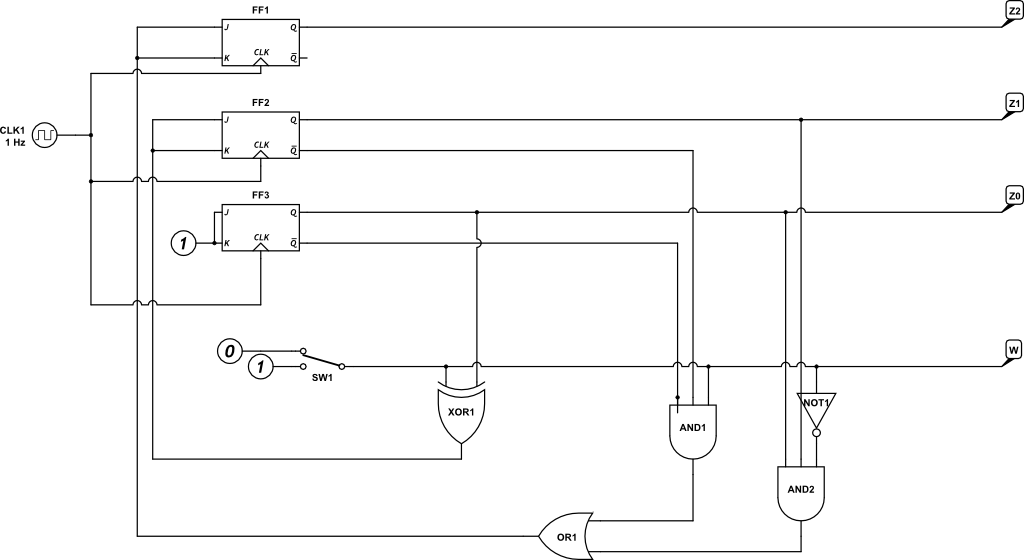
\includegraphics[width=\textwidth]{images/8_1-ringcounter-jk.png} 

\FloatBarrier
\section*{Exercise 7.2 (Flipflops)}

\subExercise{a} The state diagram for the automaton:

\begin{figure}[h]
  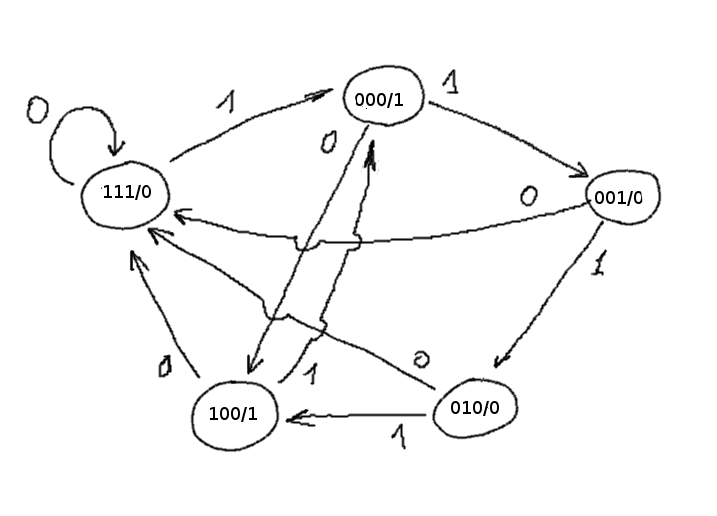
\includegraphics[width=0.5\linewidth]{images/exercise_7_2_a.png}
\end{figure}

\subExercise{b} For the implementation with D-Flip-Flops, we construct the K-Maps first
(notice that there are quite a few Don't-Care entries):
\begin{figure}[h]
  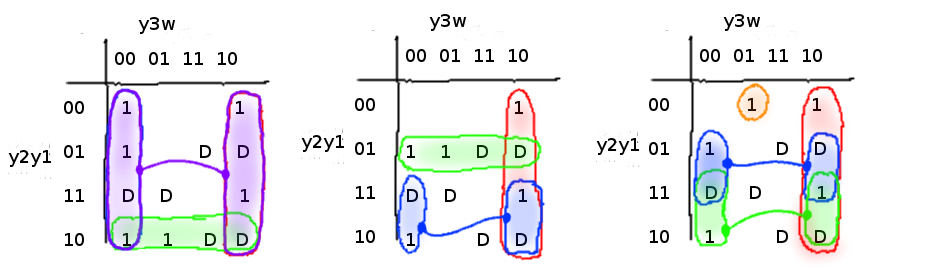
\includegraphics[width=\linewidth]{images/exercise_7_2_b.png}
\end{figure}

\noindent Possible (nearly) optimal formulas are:
\begin{align*}
  Y_3 &= \bar w + y_2 \bar y_1 \\
  Y_2 &= \bar y_3 y_1 + y_2 \bar w + y_3 \bar w \\
  Y_1 &= y_1 \bar w + y_2 \bar w + y_3 \bar w + \bar y_1 \bar y_2 \bar y_3 w
\end{align*}


\noindent This gives us the following circuit:
\begin{figure}[h]
  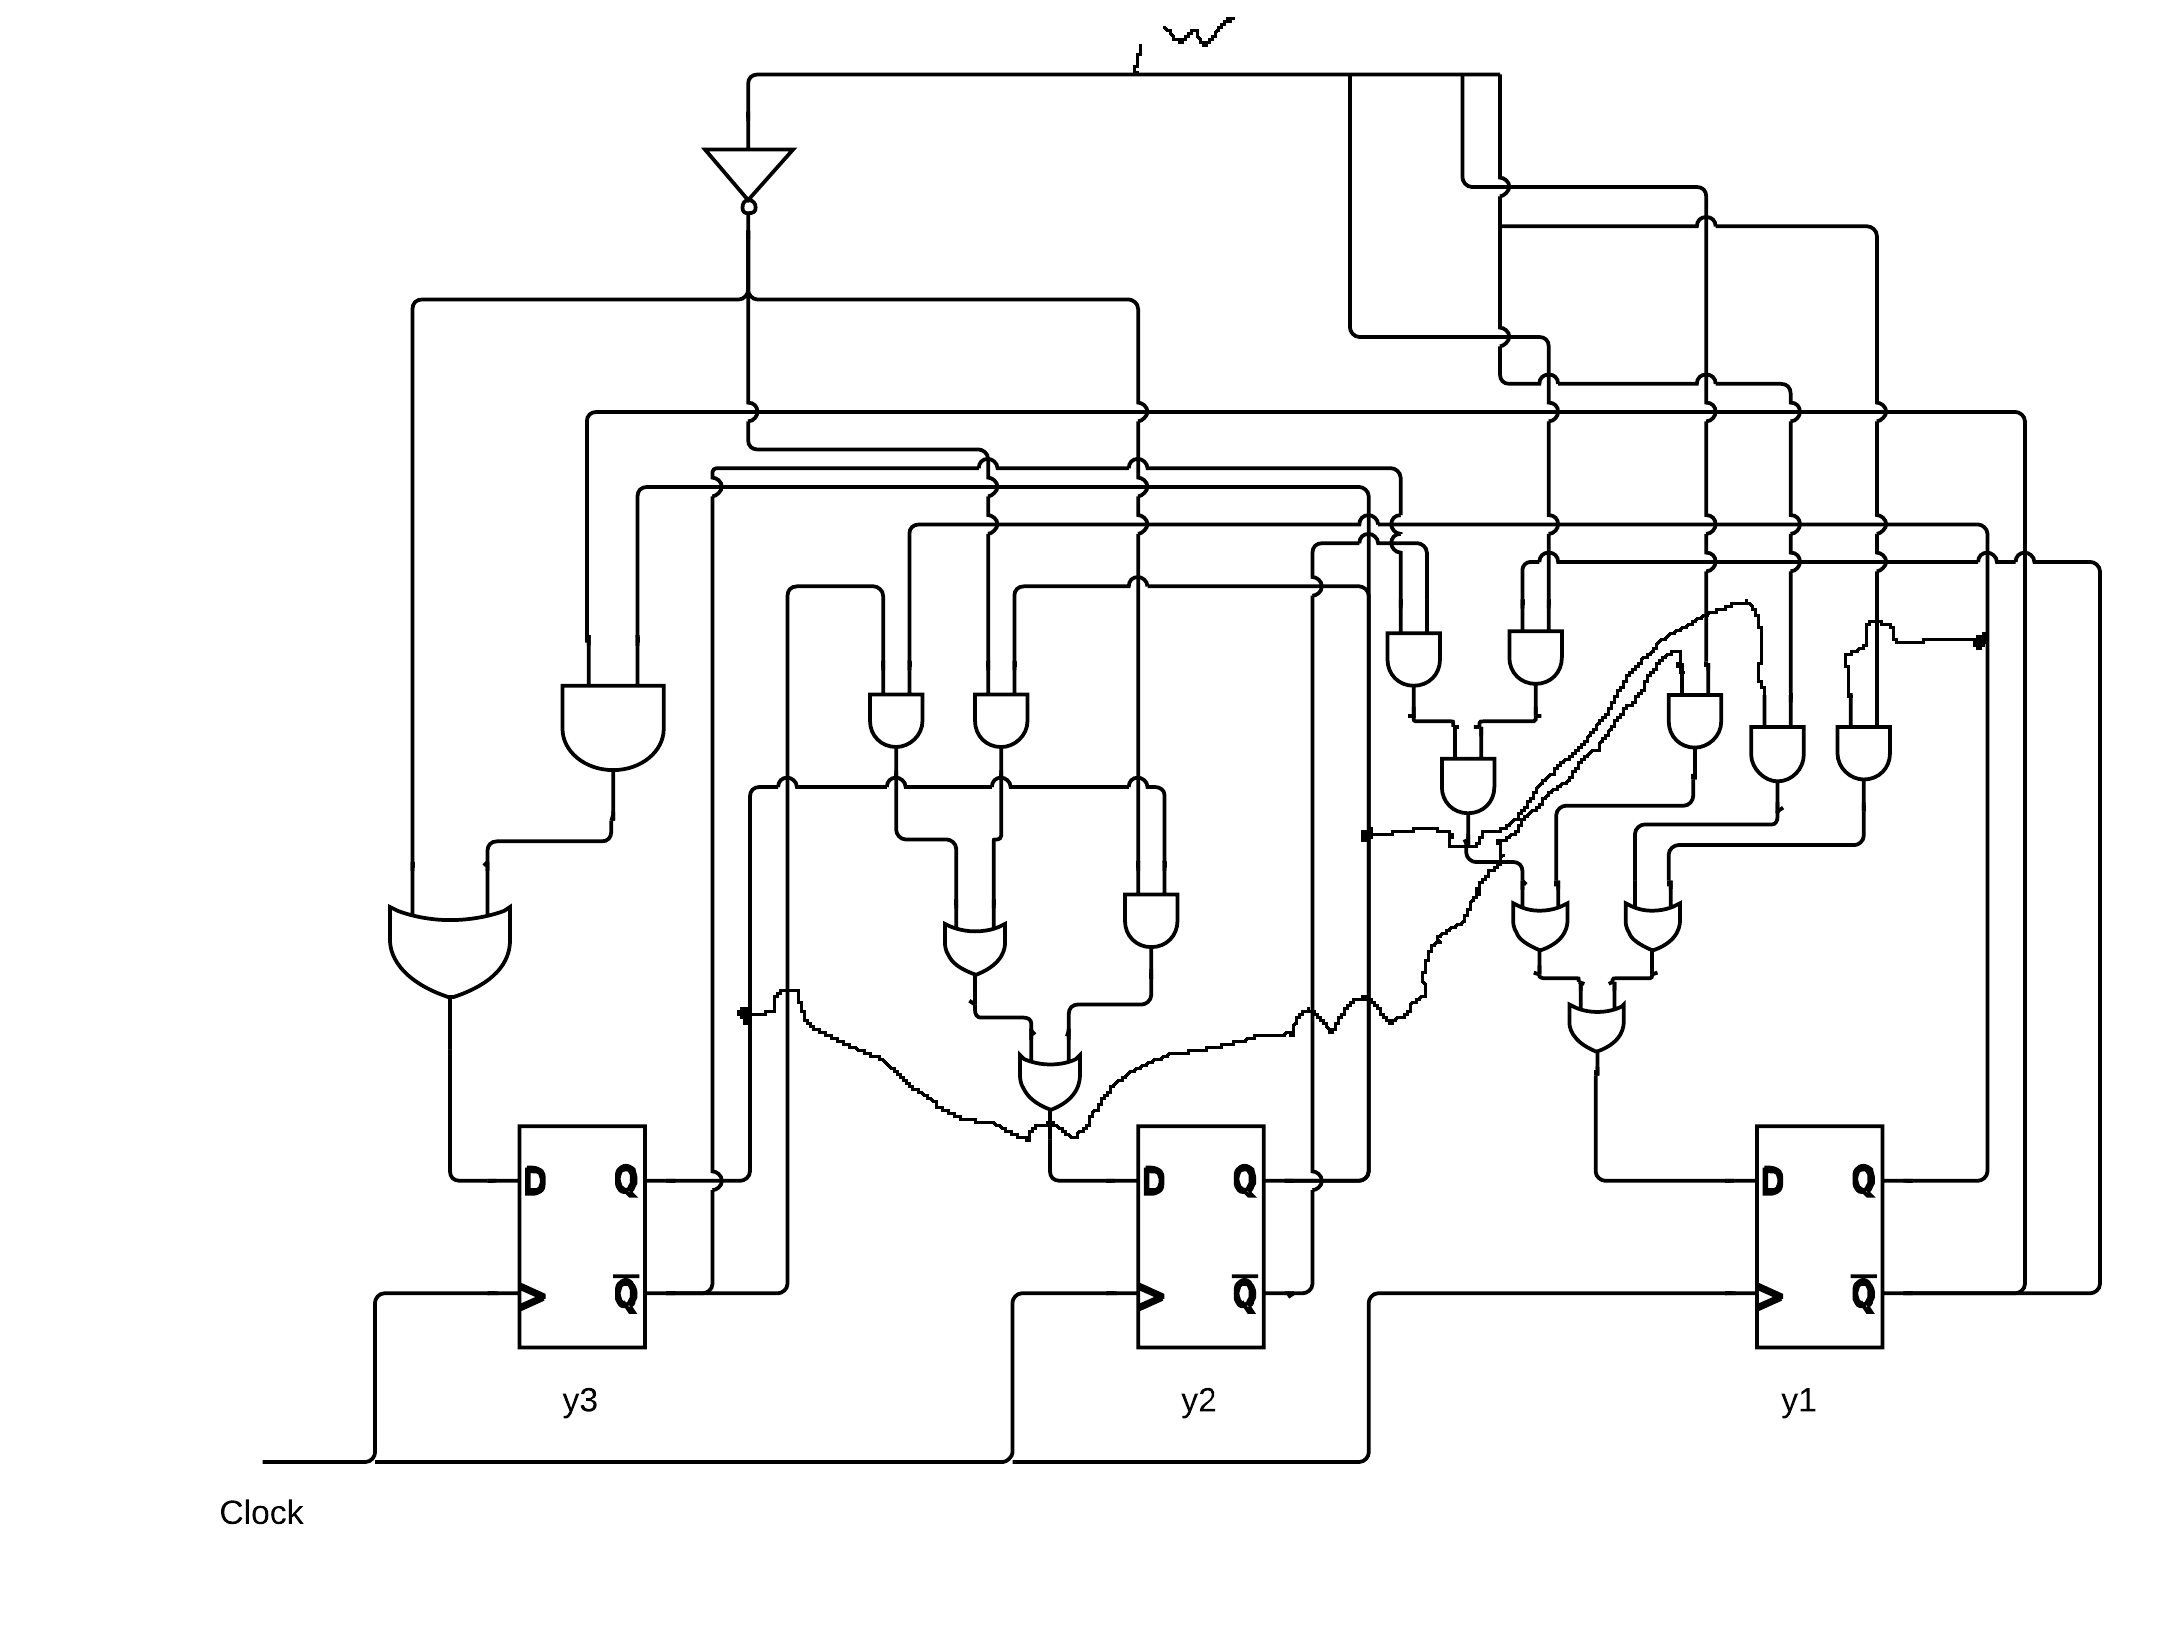
\includegraphics[width=\linewidth]{images/exercise_7_2_circuit.png}
\end{figure}

\FloatBarrier
\subExercise{c} (omitted)

\FloatBarrier
\section*{Exercise 7.3 (Gum machine)}

We contructed an automaton with 4 states, as we do not differentiate between 15 cents and 20 cents (and even more cents). (That way we have smaller tables.) 
\begin{itemize}
\item state 00 means 0 cents balance
\item state 01 means 10 cents balance
\item state 10 means 5 cents balance
\item state 11 means \glqq enough cents\grqq \ balance ( $\geq 15$ )
\end{itemize}

We have one input bit $w$, which is 0 if a 5 cent coin is insered and 1 if a 10 cent coin is inserted. That gives us the following state/output table:


\begin{tabular}{|c||c|c||c|c|}
  \hline
 State   & \multicolumn{2}{c||}{Next state} & \multicolumn{2}{c|}{Output} \\
         & $w=0$        & $w=1$            & $w=0$       & $w=1$ \\
$y_1y_0$ & $Y_1Y_0$     & $Y_1Y_0$         & $z$         & $z$   \\ \hline\hline
00       & 10           & 01               & 0           & 0     \\ \hline  
01       & 11           & 11               & 0           & 0     \\ \hline
10       & 01           & 11               & 0           & 0     \\ \hline
11       & 11           & 11               & 1           & 1     \\ \hline
\end{tabular}

We extract the K-maps for $Y_0$ and $Y_1$ and $z$ and get

\begin{tabular}{|c||c|c|c|c|}
  \hline
\textcolor{red}{$Y_0$}    & \multicolumn{4}{c|}{$y_1y_0$} \\
$w$    & 00 & 01  & 11  & 10\\ \hline\hline
  0    &    & 1   & 1   & 1 \\ \hline
  1    & 1  & 1   & 1   & 1 \\ 
  \hline
\end{tabular}
\hspace{1cm}
\begin{tabular}{|c||c|c|c|c|}
  \hline
\textcolor{red}{$Y_1$}     & \multicolumn{4}{c|}{$y_1y_0$} \\
$w$    & 00 & 01  & 11  & 10\\ \hline\hline
  0    & 1  & 1   & 1   &   \\ \hline
  1    &    & 1   & 1   & 1 \\ 
  \hline
\end{tabular}
\hspace{1cm}
\begin{tabular}{|c||c|c|c|c|}
  \hline
\textcolor{red}{$z$}   & \multicolumn{4}{c|}{$y_1y_0$} \\
$w$    & 00 & 01  & 11  & 10\\ \hline\hline
  0    &    &     & 1   &   \\ \hline
  1    &    &     & 1   &   \\ 
  \hline
\end{tabular}

$Y_0=w+y_0+y_1\qquad\qquad\qquad\qquad\quad Y_1=\bar{w}\bar{y_1} + y_0 + wy_1\qquad\qquad\qquad\quad z=y_1y_2$

and that leads us to this circuit:\\
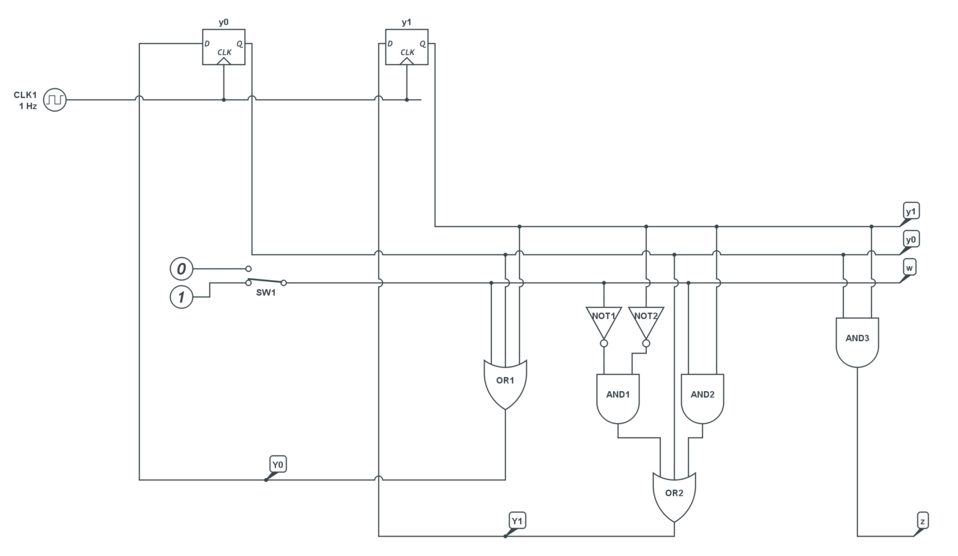
\includegraphics[width=\textwidth]{images/automat.png} 


\FloatBarrier
\section*{Exercise 7.4 (von Neumann-Adder)}
Let $A$ be a von Neumann adder with registers of size $n$.
We want to describe this adder as a finite automaton.
For this, we let $Q:=\B^n\times\B^n\times\B\times\B$ be the set of possible states, 
and interpret it as follows: 
$\textrm{accumulator}\in \B^n$, 
$\textrm{carry}\in \B^n$, 
$\textrm{highOrderBit}\in \B$,
$\textrm{moreWorkToDo}\in \B$ 
(in this order). As in the lecture and the book, we are not concerned with reading
the inputs into the registers or writing the results to somewhere else, so we set
input/output alphabets $\Sigma, \Delta = \emptyset$ and let the start state $q_0$ be
arbitrary from $\B^n\times\B^n\times\{0\}\times\{1\}$ (in the beginning, the highest
order carry-bit should not be set, and the $\textrm{moreWorkToDo}$ shall indicate 
that there is something to do).
The end states can be set to $F=\B^n\times\B^n\times\B\times\{0\}$. 
The transition function is then as follows (colon means that we prepend a zero to the tuple, empty word $\epsilon$ is omitted on both sides):
\begin{align*}
  \delta\left(
    (a_i)_{i=1}^n,
    (c_i)_{i=1}^n,
    h,
    t
  \right) 
  =
  \left(
    (a_i \not\leftrightarrow b_i)_{i=1}^n,
    0 : (a_{i-1} \wedge b_{i-1})_{i=2}^n,
    h \vee (a_n \wedge b_n),
    \bigvee_{i=2}^n(a_{i-1} \wedge b_{i-1})
  \right).
\end{align*}

Just to verify that this indeed does what we want, we implemented it literally, here is an
example of adding $568468843+708052434$ in 30-bit registers:
\begin{verbatim}
Acc:   110101101010010001000111100001
Carry: 010010111010000000101100010101
Highest bit: false
Acc:   100111010000010001101011110100
Carry: 001000010101000000000010000000
Highest bit: true
Acc:   101111000101010001101001110100
Carry: 000000001000000000000001000000
Highest bit: true
Acc:   101111001101010001101000110100
Carry: 000000000000000000000000100000
Highest bit: true
Acc:   101111001101010001101000010100
Carry: 000000000000000000000000010000
Highest bit: true
Acc:   101111001101010001101000000100
Carry: 000000000000000000000000001000
Highest bit: true
1276521277

$ echo $((568468843+708052434))
1276521277
\end{verbatim}

\end{document}

